\documentclass[tikz,border=15pt]{standalone}
\usepackage{amsmath,amssymb}
\usetikzlibrary{arrows.meta}

\begin{document}
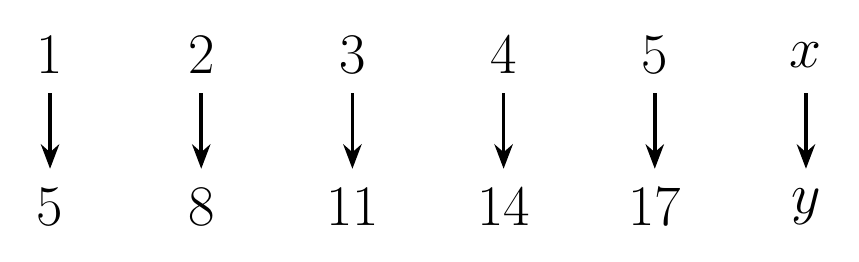
\begin{tikzpicture}[>=Stealth, scale=1.2]
    % Mapping diagram columns
    \foreach \topval/\botval/\i in {1/5/0, 2/8/1.6, 3/11/3.2, 4/14/4.8, 5/17/6.4, x/y/8.0} {
        % Top element (domain)
        \node[font=\huge\bfseries] at (\i, 1.2) {$\topval$};
        % Downward arrow
        \draw[line width=1.3pt, ->] (\i, 0.8) -- (\i, 0.0);
        % Bottom element (co-domain)
        \node[font=\huge\bfseries] at (\i, -0.4) {$\botval$};
    }
\end{tikzpicture}
\end{document}
